
Having briefly presented the theoretical concepts on which NODUS is based, the
different costs that can be assigned to the links of the virtual network remain to be analysed.
Unfortunately, and in spite of the existence of several network models,
the literature presents very few specific cost functions.  On the
following pages, cost elements already published will be discussed and commented
, in order to provide a general and concrete methodological framework,
applicable to the virtual network.

Economic analyses based on a network model are only significant if the
weights used on the different links of the network are credible.  These
weights can take different forms.  They can concern prices, costs, time
limits,... In order to be able to express these different forms of weights as
monetary values, the concept of "generalised cost" is often used, a basic
formulation of which was presented by Kresge and Roberts \footnote{Kresge, D.T.
and Roberts, P.O.,1971, "Techniques of Transportation Planning: Systems Analysis
and Simulation Models", Brooking Institution, Washington DC. A more depth discussion about generalised cost functions can be founded in Wilson A.G. and Bennet R.J., 1985, "Mathematical Methods in
Human Geography and Planning", John Wiley \& Sons, N-Y.} :

$$C_{ij}=f_{ij}+b_1s_{ij}+b_2\sigma s_{ij}+b_3w_{ij}+b_4p_{ij}$$

where:
\begin{itemize}
\item $f_{ij}$: direct costs supported by the operator between the nodes i and j
\item $s_{ij}$: travelling time between i and j
\item $\sigma s_{ij}$: variability of the travelling time
\item $w_{ij}$: waiting time before the actual transportation
\item $p_{ij}$: probability of having the shipment damaged or lost
\end{itemize}


In this formulation, the coefficients $b_n$ that balance the different
components of the function are generally proportional to the value of the
transported goods. After the example of the approach of Baumol and Vinod,
presented in an earlier chapter, the generalized cost offers the possibility to
assign a cost to all the variables influencing the traffic on a network.  This
way, a shipment expressed in kilometres or a waiting time expressed in hours can
be summed because expressed as monetary values.  The uncertain terms in those
formulations can, however, not be directly assigned on the network, except when
they are incorporated as average values.

The virtual network requires the development of four types of cost functions. As
mentioned above, the type of function is known through the notation used for the
virtual nodes. A concrete illustration is presented in table
\ref{tab4_1}.

\begin{itemize}
  \item Moving (\textbf{``mv''}): The identification numbers of the real nodes vary.
  \item Simple transit (\textbf{``tr''}): The identification numbers of the real links vary
whereas the mode and the means of transportation have remained the same.
  \item Transshipment (\textbf{``tp''}): The identification numbers of the real links vary,
as well as the mode and/or means of transportation.
  \item Loading (\textbf{``ld''}) / unloading (\textbf{``ul''}): One of the two identification numbers of the real
links is "0".
\end{itemize}



\begin{table}[htbp]
\begin{center}
\begin{tabular}{crcccrccc}
\hline


Case &Node1 &Link1 &Mode1 &Means1 &Node2 &Link2 &Mode2 &Means2\\
\hline
1 &-1000 &1000  &1 &01 &+1001 &1000 &1 &1\\

2 &+1000 &1000 &1 &01 &-1000 &1001 &1 &1\\

3 &+1000 &1000 &1 &01 &-1000 &1001 &1 &2 \\

4a &-1000 &0 &0 &0 &-1000 &1001 &1 &1\\

4b &+1000 &1001 &1 &1 &+1000 &0 &0 &0\\
\hline
\end{tabular}
\caption{\label{tab4_1} Examples of notation for virtual links}
\end{center}
\end{table}

Now, the cost elements that can be used with the different cases
remain to be determined, knowing that initially and intuitively, the total cost of
transportation can be resolved in the " accountancy " way presented in figure \ref{f4_1}:

\begin{figure}[htbp]
\centerline{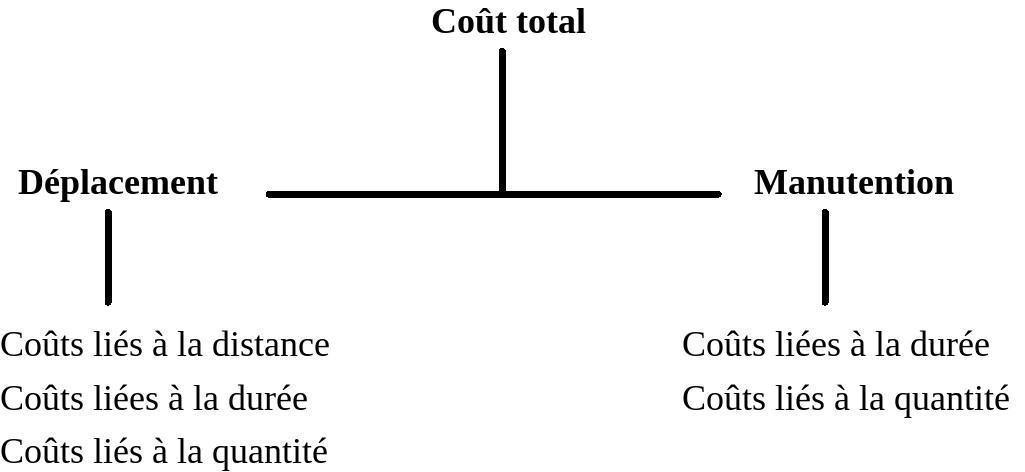
\includegraphics[width=10cm]{f4_1.png}}
\caption{\label{f4_1} Transport costs}
\end{figure}



\underline{Important remark}: It is important to keep in mind that
the functional form proposed at the end of the chapter should not be regarded as
a unique and unalterable formulation, but rather as a solution well adapted to
NODUS.  The only methodological restriction imposed by the concept of the
virtual network is the development of specific functions for the four cases
mentioned above.  The functional form of these functions can be freely chosen. Having specified this, it may be interesting to
indicate a few lines of thought, a kind of "code of good behaviour" that has to
be observed during the development of cost functions in a multi-modal
environment:



\begin{itemize}
\item Coherence of the viewpoints: a transportation can take place and be
effected by the company itself or by an independent carrier.  In the first case,
all the costs borne by the company during the transportation process have to be
analysed, whereas in the second case it is of great importance to know the
charged tariffs.  It is thus essential to adapt the same viewpoint for the
different modes of transportation taken into consideration on the network.

\item Coherence of the units: when a unit of measure is chosen (monetary units per ton, per
kilometre, per ton/kilometre,...) for a mode of transportation on a type of
virtual link, it obviously is important to use that same unit of measure for
the other modes of transportation.

\item Coherence of the variables: in the definition of the generalised costs, the same
cost factors have to be used for the different modes of transportation. If, for
instance, the duration of the trip or the financial costs are taken into
account for one mode of transportation, these same costs also have to be
introduced in the functions developed for the other modes.

\item Coherence in time: the data used in the calculations have to be time-compatible (same year of reference) for the different modes of transportation.
\end{itemize}


Having made these observations, it is possible to define a general approach of
the cost elements applicable on a virtual network.


\begin{enumerate}
\item Gathering of data while observing the principle of time-coherence
\item Development of cost functions (while observing the three other
principles of coherence)
        \begin{itemize}
        \item For all modes and means of transportation.
        \item For the four types of virtual links.
        \end{itemize}
\item Calculation of the costs on each virtual link.
\end{enumerate}

In the literature, two large categories of cost functions are
proposed.  The first one is aimed at analysing the set of costs linked to the
transportation activities.  This is an aggregated approach which, by
definition, does not apply to a network.  Unlike the first
categorie, the second type of cost functions analyses a movement from a given
origin to a given destination.  Unfortunately, this type of approach is
rather less spread, but there are certainly sufficient references to be able to
have a correct idea on the useful characteristics of transport-related costs.


The total cost of transportation consists of different parts that can be
classified in the following categories:

\begin{itemize}
\item The actual transportation: all the costs connected to the moving of
a vehicle between the points of origin and destination of the trip.

\item Inventory value: costs entailed by the storage of the goods during a certain
time span.  This part comprises real expenses such as insurances,
interest and opportunity cost (the transported goods represent a certain sum
of money, which is tied up and could have been used in another way).

\item Handling, storage: expenses linked to the manipulations of the goods beside the
actual trip.  It concerns packaging, stocking,
loading and unloading.

\item Indirect costs: costs entailed by activities subsidiary to
transport (administrative services, ...).  It is difficult to identify
these costs for a particular trip.
\end{itemize}

Besides these costs, the costs linked to congestion and the impact of the
quality of transport also need to be taken into consideration.

Congestion is indeed one of the factors influencing the cost of transportation.
It seems evident that at some moment the users of a network will encounter
congestion problems, and this has to be taken into account in the assignments.
The aim is to introduce a method able to solve the constraints linked to the
capacity of the network.

There are two fundamentally different ways to proceed:


\begin{itemize}

\item At a microscopic level, congestion leads to a slowing down of the flow and to a
choice of alternative routes to avoid traffic jams.  A solution for this
problem can be found in the network equilibrium methods that recompute the
cost functions while the flow increases.  These dynamic processes explicitly take
constraints such as the capacity of the roads or the congestion at terminals
into account.

\item At a macroscopic level, it is not always important to know whether certain
crossroads are saturated at 8 o'clock in the morning, since those crossroads are
not even introduced in the network.  However, general considerations such as the
passage through big cities or the waiting time at certain borders need to be
taken into account.  This microscopic viewpoint influences the cost functions, but
not necessarily the routes that are used.  Actually, when a large network such
as the trans-European one is digitized, the details of what is going on in a city are but rarely
dealt with.  In such a case, a digitized link can sometimes represent several
parallel routes over which the traffic will be spread over.  The cost
related to congestion can then simply be assigned to the " simple transit " virtual link in the form of a fixed cost per unit of time lost.

\end{itemize}


The quality of the transportation should be looked upon in a very broad sense
and it essentially represents the multi-products dimension of the transportation
process.  Actually, the distinction between the different products has not yet
been made, except for their inventory value.  This value, however, is not
representative since different means of transportation can be used to transport
commodities of different categories.  Imagine two types of goods of which the
weight expressed in tons is more or less the same, and which could be
transported by the same mode of transportation, but which, in practice, would be
transported by different modes of transportation and at different costs.  The
choice of the mode of transportation is thus also influenced by a certain
quality inherent to that mode and difficult to express in monetary terms.

Let us take the example of a Belgian producer exporting clothes to France.  He
chooses road transport, although it would be cheaper by
train.  A truck, however, gives him two advantages:


\begin{itemize}
\item Door to door transport;
\item Clothes are transported on hangers in the truck.
In this way, the pieces of clothing do not wrinkle.
\end{itemize}


What value should be attributed to the fact that a piece of clothing does not
wrinkle ?

Whereas factors such as time, frequence or operational safety are often found,
the concept of quality cannot that easily be introduced in a cost function.
Moreover, it is not easy to determine at what moment quality will play a role.
Is this the case while loading or while shipping ? While very interesting, this question goes 
far beyond the scope of this methodological note.

Starting from the definition of the virtual network, that requires four types of
cost functions, the table \ref{tab4_2} reflects the types of costs which
should be taken into consideration.


\begin{table}[htbp]
\begin{center}
\begin{tabular}{ll}
\hline

Type of virtual link    &Nature of the costs\\
\hline
Shipment            & Transportation\\
                    & Inventory value\\
                    & Indirects costs\\

(Un)Loading      & Handling\\
                    & Inventory value\\
                    & Indirect costs\\


Transshipment   & Handling\\
                & Storage\\
                & Inventory value\\
                & Indirect costs\\

Simple transit             & " Macroscopic " congestion \\
\hline
\end{tabular}
\caption{\label{tab4_2} Types of costs on the virtual links}
\end{center}
\end{table}

